\documentclass[10.5pt]{article}   %11 puntos

%Adapted from Adapted from UWA Engineering Final Year Project.


\usepackage[utf8]{inputenc}
\usepackage[x11names,dvipsnames,svgnames,table]{xcolor}

% general incantations
\usepackage[export]{adjustbox}
\usepackage{afterpage}

\usepackage{graphicx}
\usepackage{placeins}
\usepackage{pdfpages}
\usepackage{algorithm2e}
\usepackage{array}
\usepackage{booktabs}
\usepackage[most]{tcolorbox}
\usepackage{calligra}
\usepackage{caption}
\usepackage{datetime}
\usepackage{dirtytalk}
\usepackage{dsfont}
\usepackage{etex}
\usepackage{fancyhdr}
\usepackage{fix-cm}
\usepackage[T1]{fontenc}
\usepackage{textcomp,gensymb} %for \degree C symbol
\usepackage{graphicx}
\usepackage{lipsum}
\usepackage{listings}
\usepackage{transparent}
\usepackage[everyline=true,framemethod=tikz]{mdframed}
\usepackage{mparhack}
\usepackage{multicol}
\usepackage{multirow}
\usepackage{parskip}
\usepackage{lscape}
\usepackage{pdflscape}
\usepackage{pdfpages}
\usepackage{placeins}
\usepackage[document]{ragged2e}
\usepackage{rotating}
\usepackage{setspace}
\usepackage{subcaption}
\usepackage{threeparttable}
\usepackage[normalem]{ulem}
\usepackage{verbatim}
\usepackage{soul} %highlighting, strike through etc.

%Automated appendices
\usepackage[titletoc,title,header]{appendix} %advanced functionality

%language settings
\usepackage[utf8]{inputenc}
\usepackage{csquotes}

%page setup
%this where we adjust the binding offset, if relevant
\usepackage{geometry}
\geometry{left=2cm,right=2cm,top=2cm,bottom=2cm}
\usepackage{lastpage} % for page 1 of n footers

%cross referencing
\usepackage[hidelinks]{hyperref}
\usepackage{cleveref}

%maths stuff
\usepackage{amsmath}
\usepackage{mathtools}

\setcounter{secnumdepth}{5}

%lists
\usepackage{enumitem}

%working collaboratively
\usepackage[backgroundcolor=yellow]{todonotes}

% bibliography file using harvard
\usepackage[style=apa,citestyle=bwl-FU,backend=biber, sorting=nyt]{biblatex}
\bibliography{bibliography.bib} % with extension

%glossary for acronyms
\usepackage[acronym,nonumberlist,toc,section=subsection,numberedsection=nolabel]{glossaries} 
\makeglossaries

%line spacing
\linespread{1.6}


\usepackage{times}                      %Times New Roman
\usepackage{setspace}                   %Para espaciar
%\linespread{1.25}                      %Interlineado 1.5
%\singlespacing                          %Espaciado simple

\newcommand*\Heq{\ensuremath{\overset{\kern2pt LH }{=}}}
\newcommand{\Lagr}{\mathcal{L}}         %L (lagrangiano o fun de verosimilitud)
\newcommand{\indep}{\rotatebox[origin=c]{90}{$\models$}}
\newcommand{\R}{\mathbb{R}}             %Real numbers
\usepackage[utf8x]{inputenc}
%\usepackage{apacite}                    %Citas tipo apa
%\renewcommand{\thesubsection}{\thesection.\alph{subsection}}
%\usepackage{cite}
%\usepackage[left=2.5cm,right=2.5cm,top=2.5cm,bottom=2.5cm]{geometry} %Deberían ser 3 y 3 los left y right pero lo hago así para que entre mejor
%\usepackage[round]{natbib}              %Bibliografía
%\usepackage[utf8]{inputenc}
%\usepackage{amsmath}
\usepackage{mathtools}                  %Loads amsmath
\usepackage{amssymb}

\numberwithin{equation}{section}
\usepackage{hyperref}
\usepackage{color}   %May be necessary if you want to color links
 \hypersetup{
     colorlinks=false, %set true if you want colored links
     linktoc=all,     %set to all if you want both sections and sections linked
     linkcolor=blue,  %choose some color if you want links to stand out
 }
 \usepackage[spanish,es-tabla]{babel}
 \usepackage{graphicx}
 \usepackage{physics}
 %\usepackage[hidelinks]{hyperref}

\usepackage{amssymb}    %Para tener los check mark y cruces
\usepackage{pifont}     %Para tener los check mark y cruces
\newcommand{\cmark}{\ding{51}} %Para tener los check mark y cruces
\newcommand{\xmark}{\ding{55}}  %Para tener los check mark y cruces
\usepackage{float}

%Esto lo podés volar
% \usepackage{xcolor}                 %Night mode
% \pagecolor[rgb]{0,0,0} %black       %Night mode
% \color[rgb]{0.8,0.8,0.8} %grey      %Night mode

\title{QGIS}
\author{Matías Harari y Mariana Santi}
\date{2° trimestre 2021}
\setlength{\marginparwidth}{2cm}
\usepackage{setspace}
\spacing{1.2}
\usepackage{listings}
\usepackage{color}

\definecolor{dkgreen}{rgb}{0,0.6,0}
\definecolor{gray}{rgb}{0.5,0.5,0.5}
\definecolor{mauve}{rgb}{0.58,0,0.82}

\lstset{frame=tb,
  language=Java,
  aboveskip=3mm,
  belowskip=3mm,
  showstringspaces=false,
  columns=flexible,
  basicstyle={\small\ttfamily},
  numbers=none,
  numberstyle=\tiny\color{gray},
  keywordstyle=\color{blue},
  commentstyle=\color{dkgreen},
  stringstyle=\color{mauve},
  breaklines=true,
  breakatwhitespace=true,
  tabsize=3
}
\begin{document}
\renewcommand{\thesubsection}{\thesection.\alph{subsection}}

\thispagestyle{empty}
\setlength\headheight{0pt} 
\begin{center}

\begin{center}

\includegraphics[width=0.65\linewidth]{imgs/logoudesa.png}            
\end{center}	

        \vspace{0.2cm}
        {\scshape\LARGE Departamento de Economía \par}
        \vspace{0.2cm}
        {\scshape\Large Maestría en Economía\par}
        \vspace{0.4cm}

        {\Large\bfseries Herramientas computacionales - Python Scrapping\par}
        
        \vspace{1cm}
        {\Large\itshape Matias Harari y Mariana Santi \par}


\vspace{1cm} 
\large
{2021}

\end{center}

\clearpage
\justify


%List of figures and tables, automatic from thesis.

%\tableofcontents
%\pagebreak

%Empieza el trabajo
\section*{Crimen y clima en condados de Maryland}

En el trabajo se exploran datos de hurtos en Maryland para el año 2015. A cambio de un robo, en un hurto no existe ningún tipo de violencia o intimidación a la hora de querer apoderarse de un bien ajeno. En la Figura 1 puede verse que la relación entre hurtos y robos es alta, aunque los primeros son más usuales que los segundos.


En la Figura 1 también se presenta la relación entre la intensidad de las precipitaciones anuales (medida como el promedio anual de mm. de lluvia) y la cantidad total de hurtos cada 1000 habitantes. Una hipótesis de la literatura es que existe una relación causal negativa, ya que los días lluviosos podrían desalentar este tipo de delitos que suelen ocurrir en la vía pública. Pareciera que efectivamente se cometen más hurtos en los días menos lluviosos, aunque la relación no es fuerte. %%En este caso, la variable robo refiere específicamente a tomar un bien que está bajo la custodia de otra persona o al intento de hacerlo. 
\begin{figure}[H]
\centering
\begin{subfigure}{.5\textwidth}
    \centering
     \textbf{}\par\medskip
    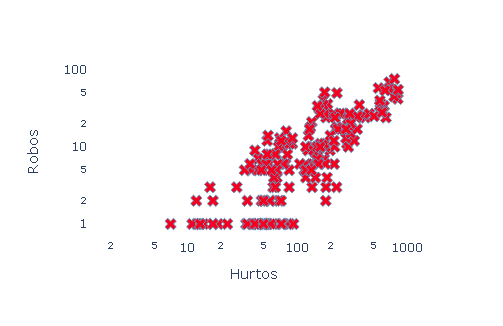
\includegraphics[scale=0.8]{robos.png}
    \label{fig2}
\end{subfigure}%
\begin{subfigure}{0.5\textwidth}
    \centering
     \textbf{}\par\medskip
    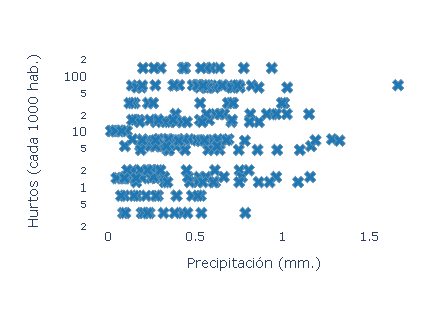
\includegraphics[scale=0.8]{plot_prec.png}
    \label{fig2}
\end{subfigure}%
\caption{Relación entre robos y hurtos (izq.) y entre precipitación y hurtos (der.) en condados Maryland. Ambos gráficos están en escala logarítmica para la variable Hurtos.}
\end{figure}

Como muestra la Figura 2, la cantidad de hurtos anuales es muy distinta entre los distintos condados. A su vez, en base a la Figura 3 se observa que algunos condados como Queen Aune's, Montgomery o Somere refuerzan la idea de una relación negativa, ya que presentan poca cantidad de hurtos y elevada cantidad de precipitación. Sin embargo, sucede lo contrario para otras ciudades como Charles, Calvert o Prince George's, que muestran una relación positiva entre las variables. Por supuesto que, para realizar un análisis más profundo, habría que mirar los datos a nivel día y no año y basarse en algún modelo econométrico.

La Figura 4 muestra el porcentaje de población de tez negra que vive en cada condado. Como hipótesis se puede conjeturar que la cantidad relativa de población negra por ciudad podría tener una relación positiva con la cantidad de hurtos debido a que las personas afroamericanas suelen insertarse en empleos de menor calificación y con menores salarios, en parte porque sufren discriminación. Por lo tanto, sería esperable que vivan en condados más pobres y con mayor inseguridad. Sin embargo, a partir de comparar las Figuras 2 y 4 no pareciera haber una relación obvia entre estas variables en el nivel de agregación anual. Es probable que un análisis más desagregado (a nivel zipcode, por ejemplo) permita dilucidar estas cuestiones de manera más clara. 



\begin{landscape}
\begin{figure}[H]
\centering
    \centering
    \includegraphics[scale=0.82]{Hurtos.png}
    \label{fig2}
\caption{Mapa de hurtos en 2015 por cada 1000 habitantes en condados Maryland.}
\end{figure}
\end{landscape}

\begin{landscape}
\begin{figure}[H]
\centering
    \centering
    \includegraphics[scale=0.82]{Lluvia.png}
    \label{fig2}
\caption{Mapa de precipitación promedio en 2015 en condados de Maryland.}
\end{figure}
\end{landscape}

\begin{landscape}
\begin{figure}[H]
\centering
    \centering
    \includegraphics[scale=0.82]{Black.png}
    \label{fig2}
\caption{Mapa de porcentaje de población negra en condados de Maryland.}
\end{figure}
\end{landscape}

\end{document}
